\section{Introdução}

    \vspace{10.5cm}

    \hspace{1cm}
    Com o advento da rede mundial de computadores, a sociedade contemporânea passou a ter facilidade no acesso a diversas fontes de informação. Sem dúvida, tal inovação contribuiu no processo de globalização das economias do século XXI. No entanto, não somente a população comum passou a produzir e consumir informações, como também agentes maliciosos tentam, frequentemente, ter acesso não autorizado a tais dados. Sendo assim, um país em busca de garantir a segurança das informações de sua população, deve adequar os crimes cibernéticos em sua constituição. Além disso, deve treinar novos especialistas para lidar com essa categoria de delito.
        
    \vspace{4mm}
    
    \hspace{1cm}
    A Forense Digital é o campo do conhecimento em que se estuda procedimentos científicos para auxiliar na investigação de crimes cometidos com o emprego de dispositivos digitais. O perito é responsável por coletar, examinar, analisar e relatar possíveis evidências encontradas em um eletrônico.
    
    \vspace{4mm}
	
	\hspace{1cm}
	Resposta a Incidentes é o ramo da Segurança da Informação especializado na procura por maneiras de mitigar ataques advindos de atores maliciosos na \textit{Internet}. Além disso, pode usar técnicas e ferramentas forenses para formalizar seu processo de investigação. Portanto, quando se fala em Forense Digital e Resposta a Incidentes (FDRI), entende-se a utilização de aparatos teórico-práticos de Forense Digital na resolução de problemas decorrentes de incidentes cibernéticos.
    
    \vspace{4mm}
	
	\hspace{1cm}
	Por meio do entendimento do processo forense clássico, percebe-se que é possível aplicá-lo na tentativa de gerar uma resposta a um ataque ocorrido. Por conseguinte, para melhor compreensão do assunto, propõe-se o estudo das seguintes subáreas de FDRI: análise de sistema de arquivos; análise de memória volátil; análise de redes de computadores; análise de logs; análise de inteligência e análise de malware.
    
    \vspace{4mm}
    
    \hspace{1cm}
    Na análise forense de sistemas de arquivos é possível entender o que estava sendo usado em um computador. Ter conhecimento de como verificar o que está contido em memória volátil é crucial para tratar casos em que criminosos utilizam este tipo de tecnologia para operar. Forense em redes de computadores é essencial para extrair informações de diferentes hospedeiros envolvidos com um incidente. A análise de logs de um sistema é pertinente para identificar eventos no mesmo. O exame de todo tipo de informação sobre um atacante é relevante para tratar com dada ameaça cibernética. Análise de malware é útil para extrair informações de programas maliciosos.
    
    \vspace{4mm}
	
	\hspace{1cm}
	Do capítulo 2 ao capítulo 7 há uma introdução a cada uma das subáreas dispostas. Ao final de cada um, há exercícios para que o leitor possa reforçar o conteúdo estudado. Dessa forma, espera-se que o aluno seja introduzido na área de FDRI. Entretanto, recomendamos que o estudante faça uma revisão de alguns conceitos de computação, através dos tópicos contidos na subseção \ref{cap1_visao_geral}.
	
   \subsection{Forense Digital}
    
    \hspace{1cm}
    Como define \citeonline{vecchia2019}, a forense digital, ou perícia forense, possui um conjunto de técnicas e procedimentos com embasamento científico para coletar, analisar e expor os indícios encontrados no processo de reconstrução de ações executadas em dispositivos digitais. Adotaremos o processo forense proposto pelo NIST, explicitado na subseção \ref{cap1_visao_geral_procfor}. Outrossim, existem tipos distintos de profissionais nesta área, e todos utilizam um método bem elaborado para efetuar uma perícia. Esta, pode ser feita em equipamentos desligados, ligados ou conectados a Internet, com as devidas ferramentas.
    
    \vspace{4mm}
        
    \hspace{1cm}
    O estudante de tecnologia da informação, que foca nessa área, pode atuar no mercado através de uma das quatro denominações de perito: oficial (passa por concurso público), \textit{ad hoc} (nomeado por um juiz), assistente técnico (contratado pelas partes envolvidas em um processo) ou privado (contratado por uma pessoa, antes de levar o caso para o judiciário). De modo a normalizar as técnicas utilizadas por esses profissionais, é adotado, internacionalmente, uma estratégia com enfoque na garantia de integridade das mídias digitais coletadas \cite{vecchia2019}.
    
    \subsection{Resposta a Incidentes} \label{cap1_ir}
    
    \hspace{1cm}
    A área de Resposta a Incidentes é aquela que realiza uma abordagem coordenada e estruturada que compreende desde a detecção de um incidente até sua resolução (resposta) \cite{luttgens2014}. Ainda, é uma profissão multidisciplinar que foca em identificar, investigar, e remediar a exploração de redes de computadores \cite{roberts2016}.

    \vspace{4mm}

    \hspace{1cm}
    Como proposto por \citeonline{luttgens2014}, para responder a um incidente, emprega-se um processo que compreende 3 etapas principais: resposta inicial, investigação e remediação. Na primeira etapa, busca-se agregar o maior número de informações sobre um incidente ocorrido. Para isso, utilizam-se informações da rede no momento do ataque, como \textit{logs} de rede \cite{luttgens2014}. Tendo identificado o incidente, as duas fases subsequentes ocorrem de forma concorrente, em busca de responder ao acometimento dos sistemas.
        
    \vspace{4mm}
    
    \hspace{1cm}
    Além das 3 etapas principais, \citeonline{luttgens2014} projetaram um processo iterativo para manutenção da fase de investigação, como mostra a figura \ref{IR_lifecycle}. Para fins didáticos, vamos nos concentrar nas subetapas de Coleta de Evidências e Análise de Dados. A coleta de evidências ocorre em função de um processo padronizado que preserva a integridade das informações. Ademais, uma organização pode modificar tal processo para atender demandas internas \cite{luttgens2014}. Como posto anteriormente, escolhemos o processo clássico do NIST para estudarmos. Finalmente, na fase de análise dos dados, busca-se extrair informações relevantes para tentar mitigar o incidente ocorrido, ao responder perguntas feitas na investigação.
    
    \begin{figure}[H]
    	\centering
    	\caption{Ciclo de vida da investigação de um incidente}
    	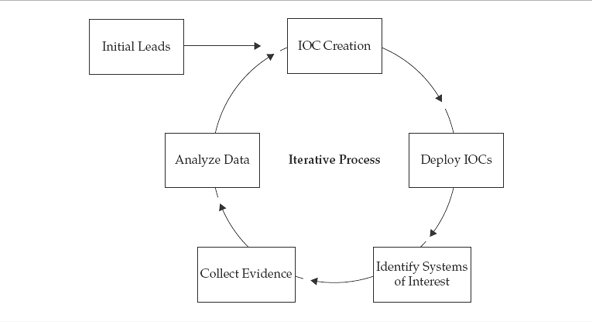
\includegraphics[scale=1]{IR_investigation}
    	\caption*{Fonte: \citeonline{luttgens2014}}
    	\label{IR_lifecycle}
    \end{figure}
    
    \subsection{Visão Geral} \label{cap1_visao_geral}
    
    \hspace{1cm}
    Antes de começar a leitura dos capítulos específicos, recomendamos que você faça uma revisão dos conceitos envolvidos com cada subárea de FDRI. Primeiramente, apresentaremos o Processo Forense Clássico proposto pelo NIST. Em seguida, explicaremos o que é Sistema de Arquivo e para que serve; o que é a Memória Principal de um computador; como são formadas as Redes de Computadores; e o que são códigos maliciosos.
    
    \subsubsection{Processo Forense Clássico} \label{cap1_visao_geral_procfor}
    
    \hspace{1cm}
    Para ser possível reconstruir as ações de um usuário em determinado dispositivo, adota-se um \textit{Processe Forense} padronizado por uma entidade de renome, para garantir que as evidências coletadas configurem um relatório pericial. Este, é então levado para uma parte interessada, que dará continuidade na investigação corrente.

    \vspace{4mm}

    \hspace{1cm}
    O \textit{Processo Forense}, internacionalmente utilizado, é aquele proposto pela entidade norte-americana NIST. Ele é constituído das seguintes etapas: Coleta, Exame, Análise e Relatório (como ilustra a imagem \ref{nist_proc}).

    \begin{figure}[H]
    	\centering
    	\caption{Processo forense clássico}
    	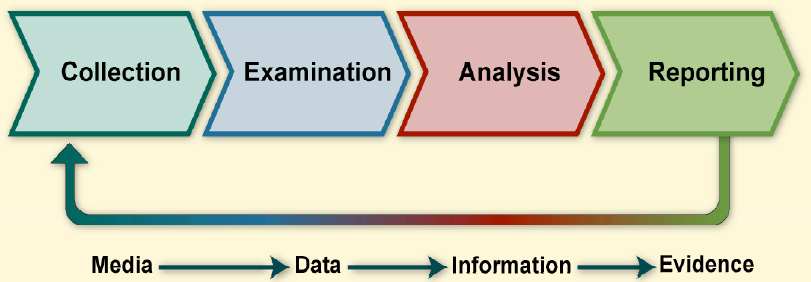
\includegraphics[scale=0.7]{nist_process}
    	\caption*{Fonte: \citeonline{kent2006}}
    	\label{nist_proc}
    \end{figure}
    
    \hspace{1cm}
    Na etapa de coleta, o profissional fará a duplicação de discos rígidos ou de memórias voláteis. Por conseguinte, inicializa-se a fase de Exame dos dados duplicados, buscando-se filtrar a grande massa de dados obtida, anteriormente, de modo a coletar informações realmente relevantes para a perícia. No estágio de análise, o perito tem que examinar, de forma manual, os resultados adquiridos na fase anterior. Essa análise é muito difícil de ser automatizada, pois, os dados devem constituir evidências para o relatório pericial. Por fim, com os resultados em mãos, o perito deve relatar tudo que foi obtido no processo \cite{kent2006}.
        
    \subsubsection{Sistema de Arquivos} \label{cap1_visao_geral_sa}
    
    \hspace{1cm}
    Todo computador pessoal é composto por um Sistema Operacional (SO) e um Sistema de Arquivos (SA). O primeiro é responsável por manter diferentes abstrações para que o usuário leigo consiga usar aplicativos em seu dia-a-dia. Já o segundo, é uma dessas abstrações, mantido  para gerir os dados do usuário, e de suas aplicações, em uma mídia de armazenamento persistente.
    
    \vspace{4mm}

    \hspace{1cm}
    Existem diversos sistemas de arquivos no mercado, cada um possui uma forma peculiar de organizar os dados do usuário em dispositivos físicos. Como o espaço destes é finito, definem-se tamanhos para cada parte armazenada pelo sistema. A menor unidade para representar informações é chamada bloco. O espaço disponível é subdividido logicamente em cabeçalho de metadados do próprio SA, e uma área de blocos de dados. Além disso, o SA também é responsável por criar as abstrações de arquivo e diretório, para o usuário final.
    
    \vspace{4mm}
    
    \hspace{1cm}
    Arquivos podem ser texto puro, codificado em algum formato como ASCII; ou \textit{bytes} armazenados para formar um arquivo binário. Alguns sistemas operacionais implementam mecanismos de identificação de tipos de arquivos, mas geralmente o cliente reconhece um arquivo pela sua extensão ou aplicação que o criou. Enquanto isso, os diretórios, ou pastas, são estruturados por meio da abstração de árvore.
    
    \vspace{4mm}
    
    \hspace{1cm}
    Todo SA implementa operações básicas para manutenção de arquivos e diretórios. O usuário comum conhece apenas as funções exibidas na interface gráfica de um SO, como criar e apagar. Porém, mais especificamente, há uma ordem lógica para manipular arquivos. Quando um dado é criado, espaço em disco precisa ser alocado, para em seguida registrar sua localização na estrutura de diretórios \cite{silberschatz2018}. Já para apagar um arquivo, o SA precisa localizá-lo na estrutura de diretórios, e então marcar seus blocos de dados como livres. Portanto, arquivos não são completamente apagados quando o usuário o deleta pela opção correspondente.
    
    \vspace{4mm}

    \hspace{1cm}
    Destacamos que os resquícios de arquivos apagados podem ser recuperados em uma análise forense por meio da técnica denominada \textit{data carving}, ou \textit{file carving} \cite{carrier2005}. Há variações de como blocos livres são gerenciados pelos SAs existentes. Mas, usualmente, programas recuperadores de dados percorrem a área de dados de um dispositivo de armazenamento, para tentar acessar blocos livres que constituem um arquivo.
    
    \subsubsection{Memória Principal}
    
    \hspace{1cm}
    Para que as aplicações do usuário final funcionem corretamente, o computador é construído utilizando uma arquitetura do conjunto de instruções de seu processador. O modelo teórico mais conhecido é a \textit{Arquitetura de Von Neumann}. Com essa abstração, o computador possui um barramento que interliga uma Unidade de Processamento Central, um módulo de dispositivos de entrada e saída de dados (E/S) e uma Memória Principal \cite{stallings2009}. Focaremos nossa revisão conceitual nessa última por enquanto.
    
    \vspace{4mm}
    
    \hspace{1cm}
    Para executar programas, o processador realiza \textit{pipelines}, mais especificamente, para buscar instruções, decodificá-las e executá-las considerando seus operadores e operandos armazenados na memória principal \cite{stallings2009}. Além desta, um processador possui memórias embutidas chamados registradores. Levando-se em consideração a hierarquia de memória organizada por \citeonline{stallings2009}, percebe-se que os registradores são mais rápidos de serem acessados pela CPU do que a memória principal. Isso se deve ao fato dessa memória transitória estar mais próxima do processador, fisicamente. No entanto, módulos de memória principal oferecem mais capacidade de armazenamento, logo, possuem papel fundamental na manutenção do mecanismo conhecido como Memória Virtual.
        
    \vspace{4mm}

    \hspace{1cm}
    De acordo com \citeonline{silberschatz2018}, a Memória Virtual é aquela encarregada de fornecer ao programador mais espaço endereçável de memória, do que seu dispositivo físico tem. Esse mecanismo aprimora o grau de multiprogramação de um computador, à medida que aparatos como paginação sob demanda e \textit{swapping} são geridos pelo sistema hospedeiro \cite{silberschatz2018}.
    
    \subsubsection{Redes de Computadores}
    
    \hspace{1cm}
    Enquanto programas são operados por usuários em computadores ao redor do mundo, no contexto de Redes de Computadores tais dispositivos são chamados sistemas finais ou hospedeiros. A rede mundial de computadores é composta por enlaces de comunicação e comutadores de pacotes. De tal maneira que um remetente consiga enviar mensagens para um destinatário, por uma rota mantida por essas equipagens.
    
    \vspace{4mm}
    
    \hspace{1cm}
    Protocolos de comunicação são empregados para garantir o funcionamento adequado da troca de mensagens pela rede. Os mais importantes são conhecidos como TCP e IP. O protocolo TCP é responsável por definir como os pacotes devem ser transportados pela rede, e o IP por criar uma hierarquia de endereçamento lógico, e repasse, para que computadores se localizem na \textit{Internet} \cite{kurose2013}. Vale ressaltar que a localização fornecida por um endereço IP não está associado a uma localização física específica no globo, mas sim a um destinatário alcançável por um remetente.
    
    \vspace{4mm}
    
    \hspace{1cm}
    O protocolo IP tem duas versões: a versão 4 e a versão 6. A primeira, também chamada IPv4, começou a ser implantada quando a \textit{Internet} surgiu, no momento em que não se previa o crescimento exacerbado do número de dispositivos a serem endereçados. Ademais, esse protocolo não garante que apenas duas partes comunicantes leiam o conteúdo de uma mensagem, tornando-se um protocolo vulnerável a ataques \textit{Man-in-the-middle}. A segunda, denominada IPv6, fora proposta para substituir sua antecedente, fornecendo criptografia no nível dos datagramas de rede, e mais combinações de endereços lógicos \cite{kurose2013}.
    
    \vspace{4mm}
    
    \hspace{1cm}
    Processos sendo executados em um hospedeiro podem se comunicar com outros sistemas finais pela rede. Para isso, emprega-se o número IP e, opcionalmente, o número de porto, ou porta. Peguemos o exemplo da ferramenta \textit{ping}. Esta implementa o protocolo ICMP que permite a um remetente enviar uma requisição \textit{echo} para um destinatário. Neste caso, o pacote de rede não é direcionado para nenhuma porta em específico, mas chega no alvo. Por outro lado, se pegarmos a \textit{Web} como caso, adota-se um nome de domínio - posteriormente traduzido em IP pelo protocolo DNS -, e o número de porto 80, para conectar clientes com sites.
    
    \vspace{4mm}
    
    \hspace{1cm}
    A democratização do acesso à informação por meio dos dispositivos móveis corroborou para o desenvolvimento das redes de computadores. Neste contexto, usuários não precisam mais de um computador de mesa, para usufruírem dos serviços fornecidos na \textit{Web}. Para que tais aplicações funcionem, existem protocolos de segurança que protegem redes sem fio. Como é o caso dos padrões WPA e WPA2, que, embora sejam vulneráveis a ataques como \textit{Evil Twin}, permitem que \textit{smartphones} de pessoas leigas se comuniquem de forma segura com o uso de algoritmos de criptografia simétrica.
    
    \vspace{4mm}
    
    \hspace{1cm}
    Todo dispositivo possui um endereço MAC de identificação. Esse valor não pode ser alterado no dispositivo, mas pode ser substituído temporariamente, para clonar o MAC de outro dispositivo. Esta técnica é usada por especialistas em redes, quando se quer obter acesso autorizado a uma rede interna que possui filtro de endereços MAC.
    
    \vspace{4mm}
    
    \hspace{1cm}
    Redes corporativas são protegidas por sistemas \textit{Firewall}. De acordo com \citeonline{kurose2013}, eles são responsáveis por isolar a rede interna da \textit{Internet}. Para isso, eles filtram pacotes de rede que entram e saem de uma sub-rede, enquanto usuários usam aplicações.

    \subsubsection{Códigos Maliciosos} \label{cap1_visao_geral_malware}

    \hspace{1cm}
    Segundo \citeonline{sikorski2012}, qualquer programa que realize alguma ação que cause danos ao seu usuário, computador ou rede pode ser considerado um código malicioso. Exemplo disso, ataques de negação de serviço, realizado com máquinas infectadas, que visam deixar um hospedeiro alvo indisponível na \textit{Internet}, através do envio massivo de pacotes de rede. 
    
    \vspace{4mm}
    
    \hspace{1cm}
    Com o emprego de programas maliciosos, atacantes podem: extorquir vítimas com o uso de \textit{ransomwares}; espionar um alvo com \textit{spywares}; enviar anúncios como spam através de \textit{adwares}; disseminar um programa malicioso chamado \textit{worm}; colocar mais \textit{malwares} no computador da vítima com o uso de \textit{trojans}, entre outros.

    \subsection{Exercícios}
    
    \begin{example}[\quad \large Introdução] \label{cap1_exercicios}
        \begin{enumerate}
            \item Quais são as etapas do Processo Forense Clássico ?
            \item Como Forense Digital e Resposta a Incidentes se relacionam ?
            \item Descreva a organização geral de um Sistema de Arquivos.
            \item Qual a importância da Memória Virtual de um computador para o usuário final ?
            \item Quais os principais protocolos de comunicação existentes na \textit{Internet} ?
            \item Defina códigos maliciosos e cite exemplos de ataques existentes.
        \end{enumerate}
    \end{example}
    
\newpage
